\documentclass[11pt]{article}
\usepackage[margin=1in]{geometry}
\usepackage{amsmath,amssymb,amsthm}
\usepackage{graphicx}
\usepackage{hyperref}
\usepackage{booktabs}
\usepackage{xcolor}
\usepackage{caption}
\usepackage{subcaption}
\usepackage{float}

\title{Finding Equilibria in Farsighted Coalition Formation:\\A Computational Search Problem}
\author{Frederik Holtel}
\date{9 June 2026}

\begin{document}

\maketitle

\section*{Context}

This work concerns a dynamic game-theoretic model of international coalition formation, developed
by Heyen \& Lehtomaa (2021) in the context of \emph{solar geoengineering governance}
\cite{heyen2021}. Solar geoengineering refers to deliberate, large-scale interventions to reduce
incoming solar radiation and thereby cool the planet. Countries differ in their preferred level of
cooling, so any deployment level will benefit some and harm others.

We focus exclusively on the \emph{power-threshold} governance regime, in which a coalition can
only deploy geoengineering if its combined power (e.g.\ economic weight) meets a minimum
threshold---say, 50\% of global power. In practice this reflects the threat of international
sanctions: a single country that attempts unilateral deployment faces sufficient economic or
political pressure from the rest of the world to be deterred. Under this regime, no individual
country can act as a ``free driver''; geoengineering deployment requires at least a two-country
coalition. The central question then becomes which \emph{coalition structures}---agreements about
who cooperates with whom---form and persist over time.

The model studies how governance rules---who can propose changes to the coalition structure, who
must consent, and what transitions are feasible---affect which structures emerge. Crucially,
countries are \emph{farsighted}: when deciding whether to join or leave a coalition, they do not
just evaluate the immediate payoff change, but anticipate the full chain of future state
transitions that their decision sets in motion.

\section{A Three-Player, Five-State Game}

The canonical illustrative case features three countries---W (Warm), T (Temperate), and C
(Cold)---with heterogeneous temperature preferences. Assuming equal power shares ($\tfrac{1}{3}$
each) and a 50\% deployment threshold, at least two countries must cooperate to deploy
geoengineering. The possible configurations of the international treaty system are captured by
five \emph{coalition structures} (states):
\begin{itemize}
  \item $(\;)$: all countries are singletons---no cooperation, no deployment ($G = 0$).
  \item $(TC)$: T and C cooperate and jointly deploy at their preferred level; W is a singleton.
  \item $(WC)$: W and C cooperate; T is a singleton.
  \item $(WT)$: W and T cooperate; C is a singleton.
  \item $(WTC)$: all three countries cooperate (grand coalition).
\end{itemize}
Each state delivers a fixed \emph{static payoff} $u_i(x)$ to every player $i$, determined by
which coalition controls geoengineering deployment and what level it chooses. Singleton countries
outside the deploying coalition have no control over the outcome and simply receive whatever
payoff the deployed level implies for them.

\subsection{The Transition Graph as a Markov Chain}

At each period, one country is selected as proposer (with equal probability $\tfrac{1}{3}$ each).
The proposer may suggest a transition to a different state; a fixed \emph{approval committee}
then votes on whether to accept. Together, these proposal and acceptance decisions determine
transition probabilities between states. Given a strategy profile $\sigma$, the resulting
transition probability matrix $P$ makes the sequence of states a \emph{Markov chain} on the
five-state space.

Figure~\ref{fig:graph} shows an example transition graph for a specific equilibrium strategy
profile: self-loops indicate the probability of remaining in the current state, and directed edges
give the probability of moving to another state in one period.

\begin{figure}[H]
  \centering
  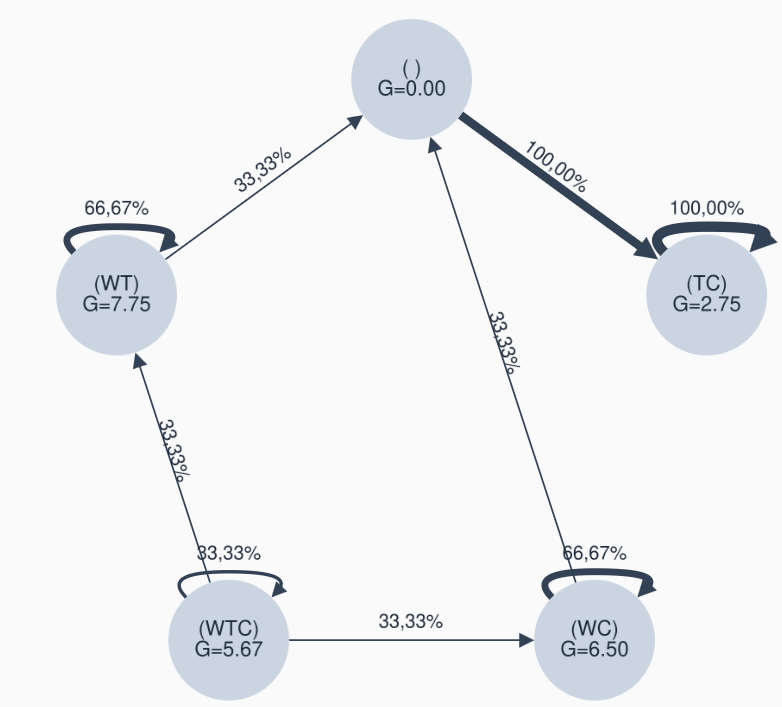
\includegraphics[width=0.65\textwidth]{sample_graph.png}
  \caption{Equilibrium transition graph for the power-threshold scenario. Node labels show the
  state name and the long-run expected payoff $G$ (geoengineering level). Edge weights are
  transition probabilities. States $(TC)$ and $(WTC)$ are absorbing under this equilibrium.}
  \label{fig:graph}
\end{figure}

\subsection{Strategy Profiles}

A \emph{strategy profile} $\sigma$ encodes two types of decisions for every player $i$, state $x$,
and possible next state $y$:
\begin{enumerate}
  \item \textbf{Proposal probability} $\sigma^P_i(x, y) \in [0,1]$: the probability that player
    $i$, when selected as proposer in state $x$, proposes a transition to state $y$. These must
    sum to one across all $y$ for each $(i, x)$.
  \item \textbf{Acceptance probability} $\sigma^A_i(x, y \mid j) \in [0,1]$: when proposer $j$
    proposes to move from $x$ to $y$, the probability that approval-committee member $i$ votes in
    favour. Only committee members have a decision here; the remaining entries are undefined.
\end{enumerate}

Table~\ref{fig:table} shows the structure of a strategy profile as used in the solver. Rows
correspond to (state, role, player) triples; columns correspond to (proposer, proposed next state)
pairs. Orange cells mark the specific decisions taken in this example; grey cells indicate entries
where the player is not in the approval committee.

\begin{figure}[H]
  \centering
  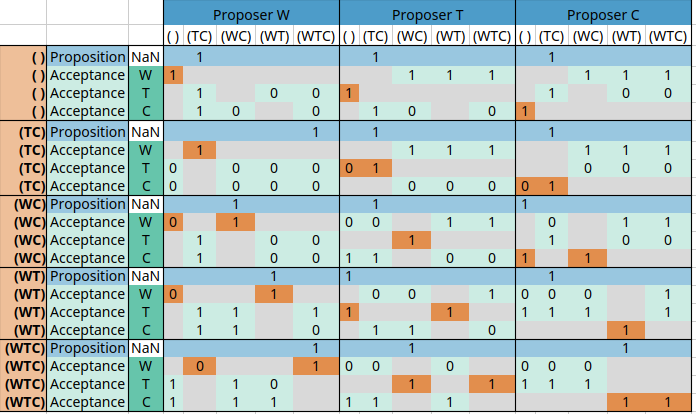
\includegraphics[width=\textwidth]{sample_strategy_table.png}
  \caption{Example strategy profile for the three-player game. Each block of rows covers one
  current state. Within each block, the first row is the proposer's probability distribution over
  next states (``Proposition''), and the remaining rows are acceptance probabilities for each
  committee member (``Acceptance''). Grey/blank cells denote entries outside the approval
  committee. This example uses \emph{pure strategies}: all entries are 0 or 1. In general,
  equilibria may involve \emph{mixed strategies} with probabilities strictly between 0 and 1.}
  \label{fig:table}
\end{figure}

The rules governing \emph{who} is in the approval committee for each transition are fixed by the
governance structure (effectivity correspondence) and are not decision variables. For example,
under unanimity rules, all current coalition members must consent to a merger; a country can
always exit unilaterally. These rules are held constant throughout the search for equilibria.

\section{The Equilibrium Conditions}

The goal is to find a strategy profile $\sigma$ that constitutes a \emph{Markov Perfect
Equilibrium} (MPE). This is not an optimisation problem in the usual sense: there is no single
objective to maximise. Instead, two rationality conditions must hold \emph{exactly
simultaneously}.

Intuitively: \textbf{players must behave rationally with respect to their long-run payoffs.} A
proposer should only suggest a transition if---taking into account the chance the committee will
approve it---the move is expected to improve their continuation value. A committee member should
approve a transition if and only if the destination state gives them a higher continuation value
than the current one. The catch is that continuation values themselves depend on the strategies:
changing who proposes what changes the Markov chain, which changes the long-run values, which
changes what is rational to propose and approve. An equilibrium is a strategy profile where these
two sides are mutually consistent.

\paragraph{Value functions.} Given a strategy profile $\sigma$ and its induced transition matrix
$P$, the \emph{Bellman continuation value} (long-run expected payoff) for player $i$ in state $x$
is the unique solution to
\begin{equation}
  V_i(x) = (1-\delta)\,u_i(x) + \delta \sum_{y} P(x,y)\,V_i(y),
  \label{eq:bellman}
\end{equation}
where $\delta \in (0,1)$ is a discount factor (typically $\delta = 0.99$). In matrix form,
$V_i = (I - \delta P)^{-1}(1-\delta)\,u_i$.

\paragraph{Condition 1 (Proposal rationality).} A proposer only puts positive probability on
transitions that maximise their expected continuation value (accounting for committee approval):
\begin{equation}
  \sigma^P_i(x,y) > 0 \;\Longrightarrow\;
  y \in \operatorname*{arg\,max}_{y'} \bigl[
    \sigma^A(x, y' \mid i)\, V_i(y') +
    (1 - \sigma^A(x, y' \mid i))\, V_i(x)
  \bigr],
  \label{eq:proposal_cond}
\end{equation}
where $\sigma^A(x,y \mid i)$ is the probability that the committee approves the proposal.

\paragraph{Condition 2 (Approval rationality).} A committee member approves if and only if the
destination state improves their continuation value:
\begin{equation}
  \sigma^A_k(x, y \mid i) =
  \begin{cases}
    1 & \text{if } V_k(y) > V_k(x), \\
    0 & \text{if } V_k(y) < V_k(x), \\
    \in [0,1] & \text{if } V_k(y) = V_k(x).
  \end{cases}
  \label{eq:approval_cond}
\end{equation}

A strategy profile is an equilibrium if and only if
equations~\eqref{eq:bellman}--\eqref{eq:approval_cond} hold simultaneously. There is no
objective function to gradient-descend; the problem is to find a \emph{fixed point} of this
coupled system.

\section{Size of the Strategy Space}

To appreciate the difficulty, consider the number of distinct binary strategy profiles (setting
each probability to $0$ or $1$):

\begin{itemize}
  \item \textbf{Proposals}: For each of the $n=3$ players and each of the $S=5$ states, the
    player proposes one of $S=5$ possible next states. This gives $5^{3 \times 5} = 5^{15} \approx
    3 \times 10^{10}$ possible proposal rules. Expressed as binary indicator variables (one bit per
    $(i, x, y)$ triple with the constraint that exactly one $y$ is chosen), there are $3 \times 5
    \times 5 = 75$ binary entries.
  \item \textbf{Acceptances}: Similarly, for each committee member, each proposed transition
    $(i, x, y)$ requires a binary accept/reject decision. The number of such entries is comparable
    to 75, summing over all relevant (proposer, current state, next state, approver) tuples.
\end{itemize}

Treating all decisions as independent binary variables gives a strategy space of size
approximately $2^{75} \times 2^{75} = 2^{150} \approx 10^{45}$. This is orders of magnitude
larger than anything approachable by brute force.

\section{Searching in the Ordinal Value Space}

Rather than searching over raw strategies, a key structural insight allows a more tractable
formulation. Under the equilibrium conditions, a player's decisions depend only on the
\emph{ordinal ranking} of continuation values $V_i(x)$ across states $x$: an approval committee
member votes yes if and only if the proposed state ranks higher, and a proposer proposes the
highest-ranked state (conditional on approval probabilities). This motivates searching over
\emph{ordinal rankings of states} per player.

Figure~\ref{fig:values} shows the continuation values $V_i(x)$ for each player $i$ and state $x$
in an example equilibrium. The equilibrium strategies are fully determined by the ordinal
structure of these values: for instance, W ranks $(CTW) \succ (CW) \succ (CT) \succ (\,) \succ
(TW)$, so W approves any transition towards $(CTW)$ and proposes it whenever selected. The
search problem reduces to finding which such ordinal ranking triple is self-consistent---i.e.\
the values induced by the corresponding strategy profile reproduce the same ranking.

\begin{figure}[H]
  \centering
  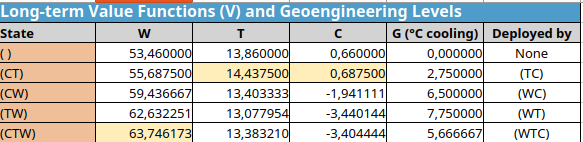
\includegraphics[width=0.82\textwidth]{sample_longterm_values.png}
  \caption{Long-run continuation values $V_i(x)$ and geoengineering deployment levels for each
  state $x$ and player $i \in \{W, T, C\}$ in an example equilibrium. The equilibrium conditions
  depend only on the \emph{ordinal} ranking of these values within each row (per player): which
  state a player prefers to be in determines both approval and proposal behaviour. Highlighted
  cells mark values that are decisive for a player's ranking.}
  \label{fig:values}
\end{figure}

\paragraph{Strict ordinal rankings.} For $n = 3$ players and $S = 5$ states, there are $5! = 120$
strict rankings (permutations) per player, giving a search space of
\[
  (5!)^3 = 120^3 = 1{,}728{,}000 \approx 1.7\text{M}
\]
triples of rankings to examine. For each triple, one can: (1) induce a strategy profile
deterministically, (2) compute $V$ via the linear system~\eqref{eq:bellman}, and (3) verify
whether conditions~\eqref{eq:proposal_cond}--\eqref{eq:approval_cond} hold. This is exhaustively
feasible.

\paragraph{Weak ordinal rankings (allowing ties).} Since value ties are possible (two states
may deliver the same continuation value to a player), one must also consider \emph{weak orders},
where ties between states are permitted. The number of weak orders on $S=5$ states is given by
the ordered Bell (Fubini) number $a(5) = 541$. The resulting search space is
\[
  541^3 = 158{,}340{,}421 \approx 150\text{M}.
\]

\paragraph{Computational cost.} A full exhaustive search over the $\approx 150$M weak-order
triples takes up to \textbf{24 hours} on a 2-CPU virtual machine. For larger games---e.g. $n = 4$ players, $S = 15$ states, or $n = 5$
players, $S = 52$ states---the search space grows as $\bigl(a(S)\bigr)^n$ and quickly becomes
intractable.

\paragraph{Density of equilibria.} In practice, for the three-player scenarios studied, the
search typically finds \textbf{1--10 equilibria} among the $\approx 150$M candidates. The density
is thus on the order of $10^{-7}$, making random sampling highly unlikely to succeed.

\section{The Core Algorithmic Challenge}

The exhaustive ordinal-ranking search solves the problem for $n = 3$, but does not scale. The
natural alternative is an iterative fixed-point algorithm:
\begin{enumerate}
  \item Start from an initial strategy profile $\sigma^{(0)}$ (e.g.\ random or uniform).
  \item Compute continuation values $V^{(t)}$ from $\sigma^{(t)}$ via~\eqref{eq:bellman}.
  \item Update the strategy profile $\sigma^{(t+1)}$ to be rational given $V^{(t)}$
    (i.e.\ apply conditions~\eqref{eq:proposal_cond}--\eqref{eq:approval_cond}).
  \item Repeat until convergence.
\end{enumerate}
The difficulty is that this iteration has no guaranteed convergence properties. In practice, it
frequently \emph{cycles}: the strategy update at step 3 changes $P$, which changes $V$, which
changes the rational strategy, which may return to a previously visited profile without ever
reaching a fixed point. Smoothed/softmax approximations (replacing hard argmax and step functions
with temperature-parameterised soft versions, followed by annealing) partially mitigate cycling
but are unreliable, particularly for larger $n$ or scenarios with a sparse equilibrium structure.

\medskip

\noindent\textbf{Open question.} We are looking for a principled algorithm---possibly iterative,
possibly based on branch-and-bound, mixed-integer programming, or other techniques from
reinforcement learning or game-theory computation---that can:
\begin{itemize}
  \item Certifiably find \emph{one} or \emph{all} equilibria for a given game instance,
  \item Scale to at least $n = 4$--$5$ players, and
  \item Handle the fixed-point structure of the problem without cycling.
\end{itemize}
The problem has similarities to finding Nash equilibria in stochastic games, value iteration in
MDPs with endogenous transition kernels, and feasibility problems in complementarity
programming---but the specific structure of endogenous Markov transitions, coupled proposal and
approval decisions, and the ordinal rationality conditions makes it non-standard.

\begin{thebibliography}{9}
\bibitem{heyen2021}
  D.~Heyen and J.~Lehtomaa,
  ``Solar geoengineering governance: A dynamic framework of farsighted coalition formation,''
  \emph{Oxford Open Climate Change}, vol.~1, no.~1, 2021.
\end{thebibliography}

\end{document}
